\documentclass[]{article}
\usepackage{fullpage}
\usepackage{amsfonts}
\usepackage{amsmath}
\usepackage{graphicx}

\begin{document}

	\title{MAT 1320}
	\author{{\bf Calculus I}}
	\date{2013}
	\maketitle
	\begin{center}
		{\bf Prof:} Paul-Eug\`{e}ne Parent
	\end{center}
	\pagebreak
	\normalsize 
	\noindent{\bf Notations and symbols}\\

	\noindent Let $a\in\mathbb{R}$. We defined the \emph{absolute value} of $a$ by:
	$$
		 |a|:=\begin{cases}
			a\text{ if } a>0\\
			-a\text{ if }a<0
		\end{cases}
	$$
	\emph{Note: $:=$ is the "definition" sign.}\\
	The result is always a positive number.
	\begin{itemize}
		\item $|0|=0$
		\item $|3|=3$
		\item $|-2|=2$
		\item $|\sqrt{2}-1|=\sqrt{2}-1$
	\end{itemize}
	{\bf Properties of the absolute value}
	\begin{itemize}
		\item $|ab|=|a||b|$
		\item if $b\ne 0$, then $|\frac{a}{b}|=\frac{|a|}{|b|}$
	\end{itemize}
	If $a>0$, then
	\begin{itemize}
		\item Solve $|2x-5|=3$
		\item {\bf Solution:} We have two cases to consider:\\
		$2x-5=3$, which leads to $x=4$,\\
		$-(2x-5)=3$, which leads to $x=1$\\
		Hence the result: $x=1$ or $4$
		\item Solve $|3x+2|\ge 4$\\
		Either $3x-2>4$, which leads to $x\ge\frac{2}{3}$\\
		Or $3x+2\le -4$, which leads to $x\le -2$\\
		Hence the result $x\in ~]-\infty,-2]\cup[\frac{2}{3},+\infty [$
	\end{itemize}
	{\bf Small remarks on the square root function:}\\
	By definition, its \emph{domain}, i.e. the allowed numbers that can feed into the quare root, is
	$$x\in~[0, +\infty[$$
	While its \emph{range}, i.e. what values the square root can "spit out", is
	$$y\in~[0,+\infty[$$
	We usually encompass all this information in a neat, compact form, i.e.:
	$$\sqrt{\cdot}:~[0,+\infty[~\rightarrow~[0,+\infty[$$
	$$x\mapsto\sqrt{x}$$
	Where the second line gives the actual transformation recipe.
	\pagebreak\\
	We can extend this to all functions, i.e.
	$$f:D\longrightarrow R$$
	$$x\mapsto f(x)$$
	Where we recover at once on the first line the name of the function $f$, its domain $D$, and its range $R$, while the second line gives us the explicit transformation rule.\\
	Ex:
	$$g:\mathbb{R}\longrightarrow\mathbb{R}$$
	$$x\mapsto x^3\cdot\sin(x)=g(x)$$
	That being said, what is:
	$$\sqrt{a^2}=|a|$$
	The range of a square root function is always $[0,+\infty[$. Indeed... $\sqrt{(-3)^2}=\sqrt{9}=3=|-3|$\\
	The square root function \emph{is a one-to-one function}.\\
	$$|a|=\sqrt{a^2}$$
	\pagebreak\\
	{\bf Recall}\\
	We will denote a function $f$ by
	$$f:D\rightarrow R$$
	$$x\mapsto f(x)$$
	Where $D$ is the domain of $f$, $R$ is its range, and $f(x)$ is the actual transform rule.\\\\
	{\bf Definition}\\
	The \emph{image} of $f$, denoted $f(D)$, is the set of all $y\in R$ such that there exists at least one $d\in D$ with
	$$f(d)=y$$
	\underline{Example:} Consider the squaring function:
	$$(\cdot)^2:\mathbb{R}\rightarrow\mathbb{R}$$
	$$x\mapsto  x^2$$
	This leads to\\
	{\bf Definition}\\
	A function is onto (ur surjective) if its image is equal to its range.\\
	\underline{Examples}:
	\begin{itemize}
		\item $x^2$ is not onto
		\item $x^3$ is onto
	\end{itemize}
	\begin{center}
		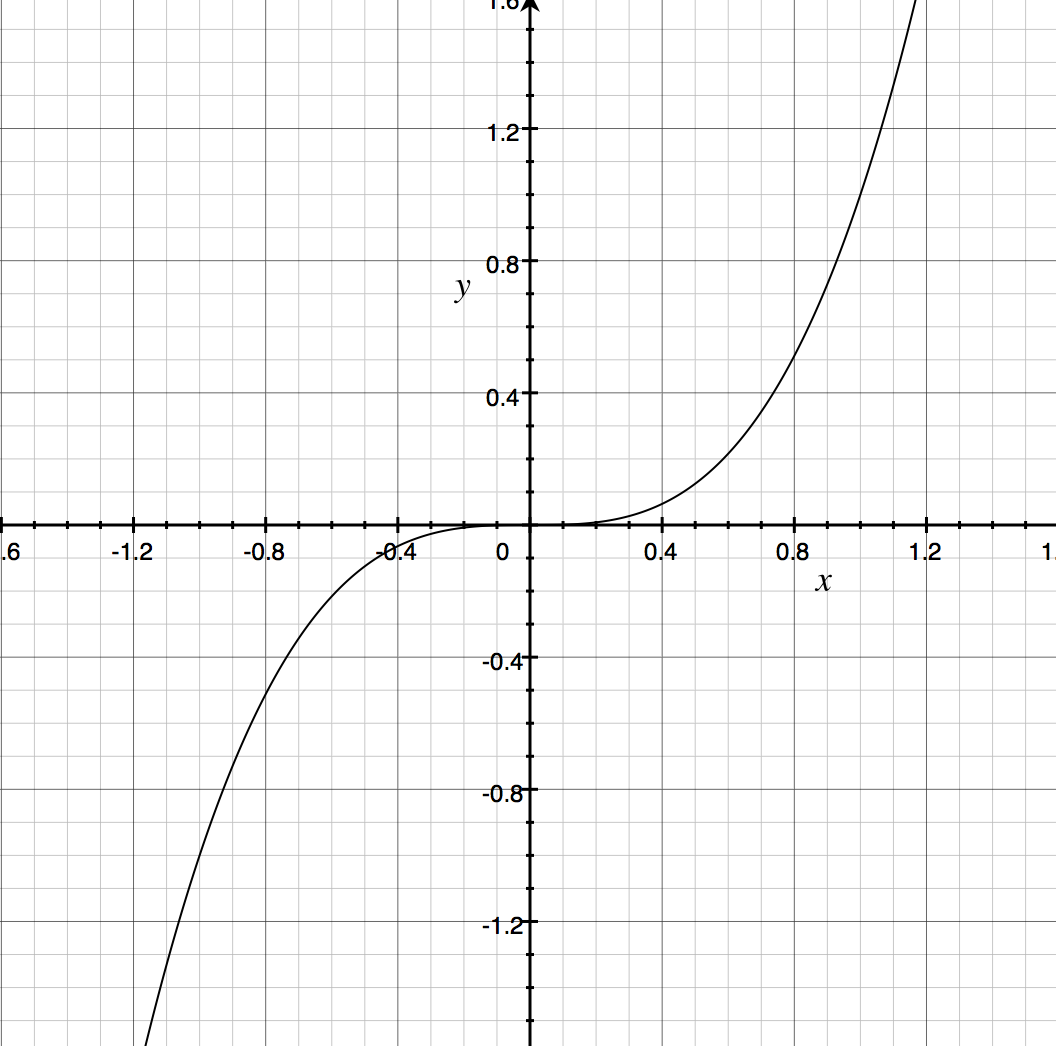
\includegraphics[scale=0.4]{./graphics/x3.png}\\
		\emph{The function, $x^3$}\\
	\end{center}
	{\bf Definition}\\
	A function is \emph{one-to-one} or \emph{injective} if whenever $f(x_1)=f(x_2)$, we then must have $x_1=x_2$.\\
	In other words, a one-to-one function cannot produce more than once a given value.\\
	\underline{Examples:}\\
	\begin{itemize}
		\item The squaring function is {\bf not} one-to-one because\\
		$(-2)^2=2^2$ but $-2\ne 2$
		\item The cubic function is one-to-one.
	\end{itemize}
	If a function $f$ is both onto \emph{and} one-to-one, it's called a \emph{bijection}.\\
	{\bf Theorem}\\
	A function $f:A\longrightarrow B$ is a bijection if and only if there exists a function $f^{-1}:B\longrightarrow A$ such that:
	\begin{itemize}
		\item $f^{-1}(f(a))=a$ for all $a\in A$, and
		\item $f(f^{-1}(b))=b$ for all $b\in B$
	\end{itemize}
	{\bf Remarks:}\\
	\begin{itemize}
		\item If such  a function exists, then it is unique. It is called the inverse of $f$.
		\item We must have
		$$b=`f(a) \iff a=f^{-1}(b)$$
		\item\underline{\bf WARNING:}
		$$f^{-1}(x)\ne\frac{1}{f(x)}$$
		$$(f(x))^{-1}=\frac{1}{f(x)}$$
	\end{itemize}
	\underline{Example}\\
	Find the inverse of $f(x)=x^3+2$.\\
	\underline{Solution}
	\begin{itemize}
		\item Write $y=x^3+2$
		\item Solve for $x$ as a function of $y$, i.e.
		\begin{itemize}
			\item $x^3=y-2$ hence $x=(y-2)^{1/3}$
		\end{itemize}
		\item Switch $x$ and $y$, i.e. $y=(x-2)^{1/3}$
	\end{itemize}
	Checking computations with...
	\begin{itemize}
		\item$f(f^{-1}(x))=f((x-2)^{1/3})\\
		=((x-2)^{1/3})^3+2\\
		=x-2+2=x$
	\end{itemize}
	The function $\sqrt{x}$ is not the inverse of $x^2$.\\
	Recall that $\sqrt{x^2}=|x|$ and not $x$ is neither one-to-one nor onto, and hence is not invertible!\\\\
	But we can consider a new function with a smaller domain and a smaller range but with the same transformation rule.
	$$h:~[0,+\infty[~\longrightarrow~[0,+\infty[$$
	$$x\mapsto x^2$$
	Now that function is a bijection and its inverse is $\sqrt{x}$, i.e. $\sqrt{h}=x$ and $(\sqrt{x})=x$
	\pagebreak\\
	\Large{Logarithms}\\
	\normalsize{\bf Remarks:}\\
	1. $f_a$ is hence one-to-one, and\\
	2. If we restrict the range of $f_a$ to $]0,+\infty[$, then$f_a$ becomes a bijection.\\
	We denote ints inverse by
	$$\log_a(x)$$
	The number $a$ is called the base\\
	If the base is omitted as in $\log 5$, it is assumed to be base 10\\
	When $a=e\approx 2.71828$, the log is written
	$$\ln(x)$$
	Recall that for $1\ne a>0$ we have the exponential function:
	$$f_a:\mathbb{R}\longrightarrow\mathbb{R}$$
	$$x\mapsto a^x$$
	which is 
	\begin{itemize}
		\item strictly decreasing if $a>1$; and
		\item strictly increasing if $a<1$.
	\end{itemize}
	\underline{Remarks}:\\
	1. $f_a$ is hence one-to-one, and\\
	2. $f_a(x)>0$.\\
	Hence if we restrict the range of $f_a$ to $]0,+\infty[$, then $f_a$ becomes a bijection.\\
	We denote its inverse by $log_a(x)$\\
	This function is characterized by:
	$$
	log_a(x)=y\iff a^y=x
	$$
	\begin{itemize}
		\item The number $a$ is called the \emph{base}
		\item If the base is omitted as in $log(5)$, it is assumed to be 10.
		\item When $a=e\approx 2.71828$, we write $\ln(x)$, and we call it the natural logarithm.
	\end{itemize}
	\begin{center}
		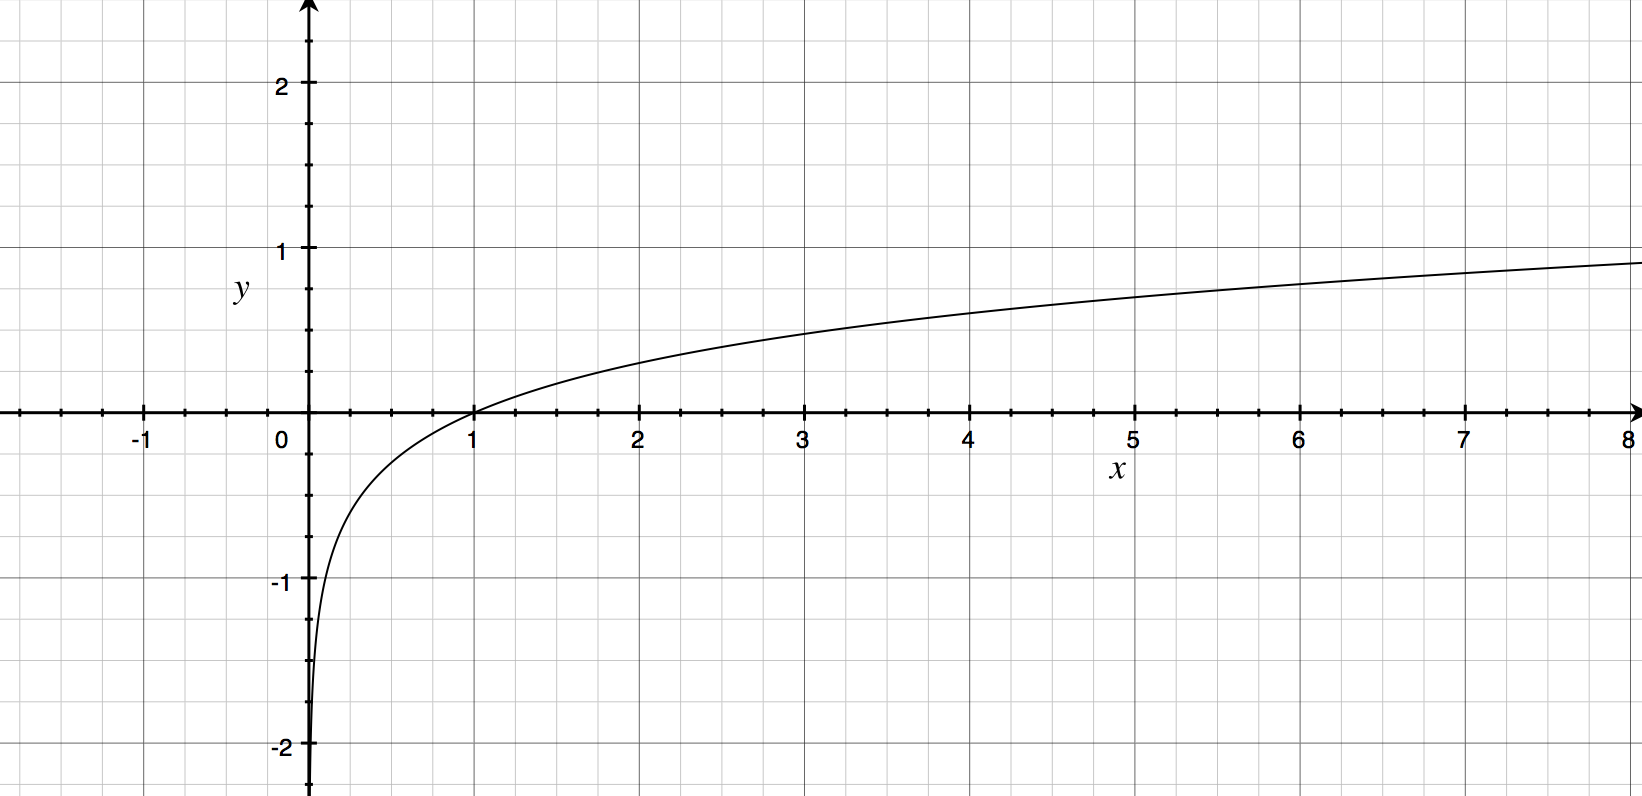
\includegraphics[scale=0.4]{./graphics/logx.png}\\
		\emph{$\log(x)$}
	\end{center}
	Compute $\log_2(80)-\log_2(5)$
	\begin{align*}
		\log_2(80)-\log_2(5)&=\log_2\frac{80}{5}\\
		&=\log_2(16)\\
		&=4
	\end{align*}
	Theorem:\\
	Let $1\ne a>0$ and $x>0$. Then:
	$$\log_a(x)=\frac{\ln(x)}{\ln(a)}.$$
	Why is this true?\\
	If $y=\log_a(x)$, then $a^y=x$. Applying $\ln$ to both sides we get:
	$$
	\ln(x)=\ln(a^y)=y\ln a.
	$$
	Hence $y=\frac{\ln(x)}{\ln(a)}$.\\\\
	Compute with a precision of six decimal places
	$$
	\log_8(5).
	$$
	\underline{Solution:} $\log_8(5)=\frac{\ln(5)}{\ln(8)}\approx 0.773976$\\\\
	Solve $e^{5-3x}=10$\\
	\underline{Solution:}\\
	Apply $\ln$ to both sides\\
	Solve for $x$, i.e. $x=\frac{5-\ln(10)}{3}\approx 0.899138$\\\\
	\pagebreak\\
	\Large{Trigonometry}\\
	\large{Inverse trig functions}\\
	\normalsize
	Consider a circle of radius $r$ and some arc of length $a$ and $c$ its circumference.\\
	On a unit circle,
	\begin{itemize}
		\item A(0)=(1,0) implies $\cos(0)=1$ and $\sin(0)=0$
	\end{itemize}
	{\bf Properties}\
	The function $A(\theta)$ is periodic of a period of $2\pi$, i.e. $A(\theta)=A(\theta+2\pi)$. Hence:
	$$
	\cos(\theta)=\cos(\theta+2\pi)\text{ and }\cos(\theta)=\cos{\theta-2\pi}
	$$
	As one can deduce by either their respective definitions or their associated graphs,
	\begin{itemize}
		\item The function $\sin\theta$ is an odd function
		\item The function $\cos\theta$ is an even function
	\end{itemize}
	\begin{center}
		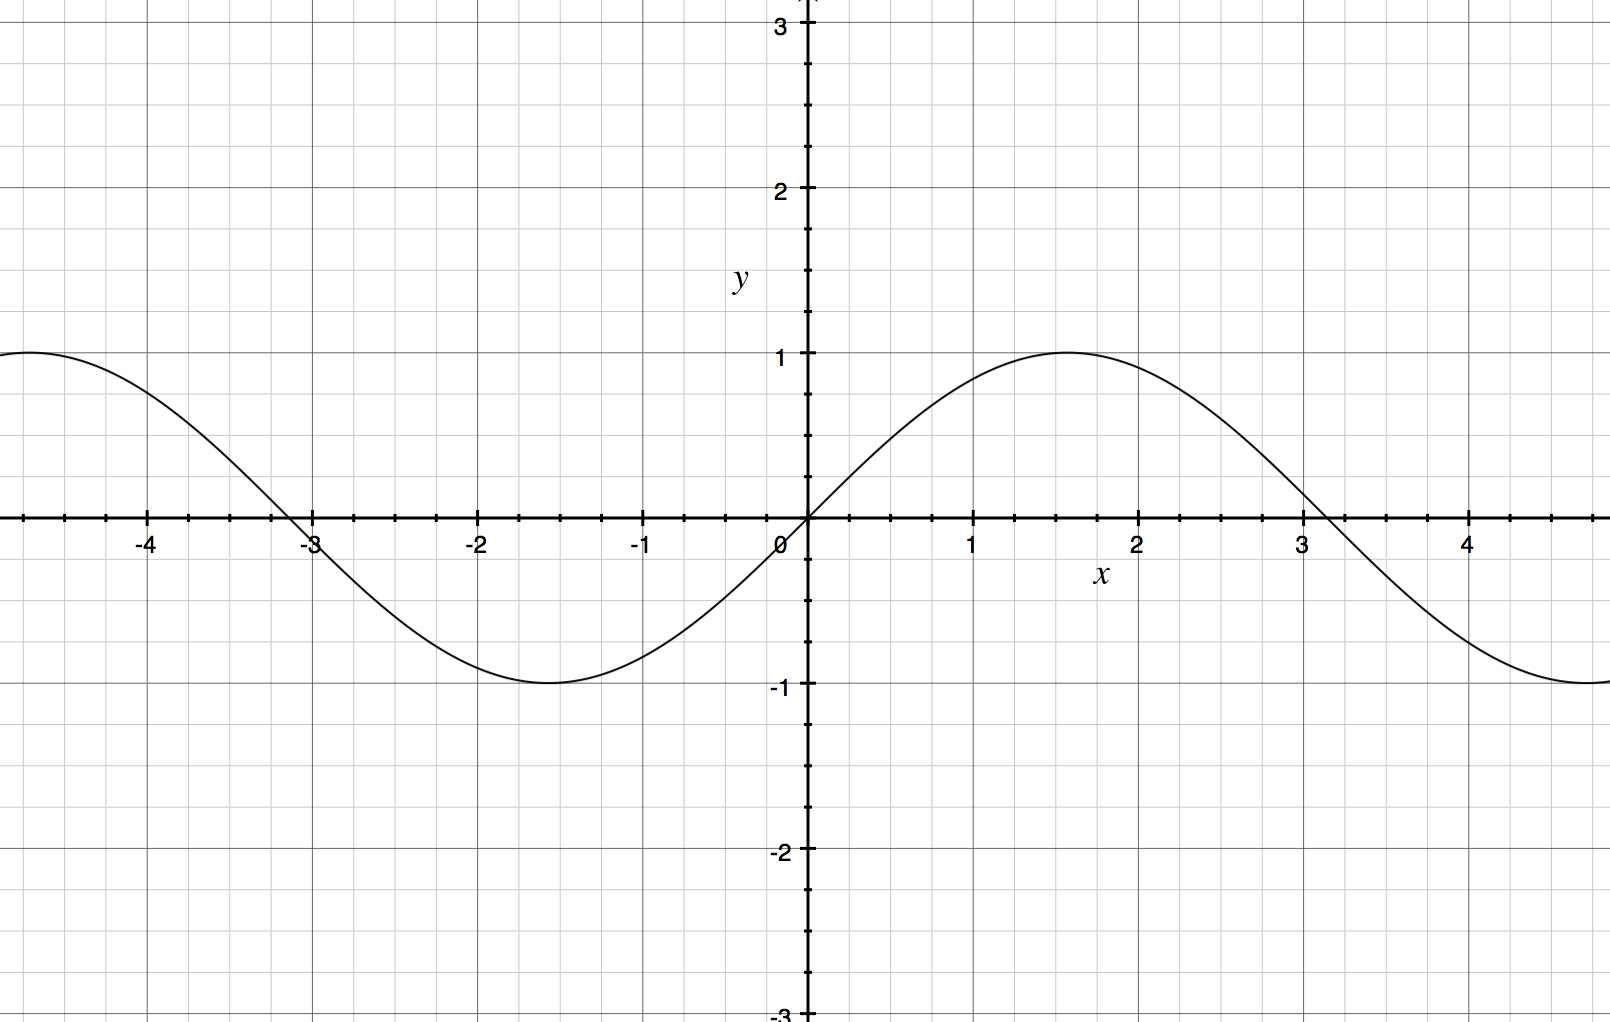
\includegraphics[scale=0.4]{./graphics/sinx.png}\\
		$\sin(x)$
	\end{center}
	{\bf Other trig functions}
	$$
	\tan(\theta):=\frac{\sin(\theta)}{\cos{\theta}}\text{ and }\cot{\theta}=\frac{\cos(\theta)}{\sin(\theta)}
	$$
	\begin{center}
		Secant and cosec
	\end{center}
	From $\cos^2(\theta)+\sin^2(\theta)=1$ one can define:\\
	$1+\tan^2(\theta)=\sec^2(\theta)$\\\\
	{\bf To do at home: }
	Show that:\\
	\begin{itemize}
		\item $\sin(2x)=2\sin(x)\cos(x)$
		\item
			\begin{align*}
				\cos(2x)&=\cos^2(x)-\sin^2(x)\\
				&=2\cos^2(x)-1\\
				&=1-2\sin^2(x)
			\end{align*}
	\end{itemize}
	\pagebreak
	Find all $x\in[0,2\pi]$ such that $\sin(x)=\sin(2x)$\\
	\underline{Solution:} Recall that $\sin(2x)=2\sin(x)\cos(x)$, hence we need to solve\\
	$\sin(x)=2\sin(x)\cos(x)$. Equivalently, $\sin(x)(1-2\cos(x))=0$.\\
	We have two cases:
	\begin{itemize}
		\item $\sin(x)=0$, which implies that $x=0, \pi, or 2\pi$, or
		\item $1-2\cos(x)=0$, which implies $\cos(x)=\frac{1}{2}$, or equivalently $x=\frac{\pi}{3}$ or $\frac{5\pi}{3}$
	\end{itemize}
	Conclusion: The solutions are $x=0,\frac{\pi}{3},\pi,\frac{5\pi}{3},$ or $2\pi$\\\\
	We want to "invert" the trigonometric functions. Recall that the domain and the range of $\sin(x)$ and $\cos(x)$ are the real numbers. Two problems arise:
	\begin{itemize}
		\item both functions are periodic, hence they are not one-to-one
		\item both functions are not onto as their images are $[-1,1]$
	\end{itemize}
	We then need to consider \emph{restricted} versions of those functions if we want to proceed.\\
	In the case of $y=\sin(x)$, we consider the classical domain 
	$$[-\frac{\pi}{2},\frac{\pi}{2}]\longrightarrow[-1,1]$$
	$$x\mapsto\sin(x)$$
	Hence the function $y=Sin(x)$ is now onto and one-to-one and thus admits and inverse function
	$$
	\arcsin~:~[-1,1]\longrightarrow[-\frac{\pi}{2},\frac{\pi}{2}].
	$$
	In particular,\\
	\begin{itemize}
		\item $\arcsin(Sin(x))=x~\forall~x\in[-\frac{\pi}{2},\frac{\pi}{2}]$
		\item $Sin(\arcsin(x))=x~\forall~x\in[\frac{-1}{1}]$
		\item $y=\arcsin(x)\iff Sin(y)=x$
	\end{itemize}
	\begin{center}
		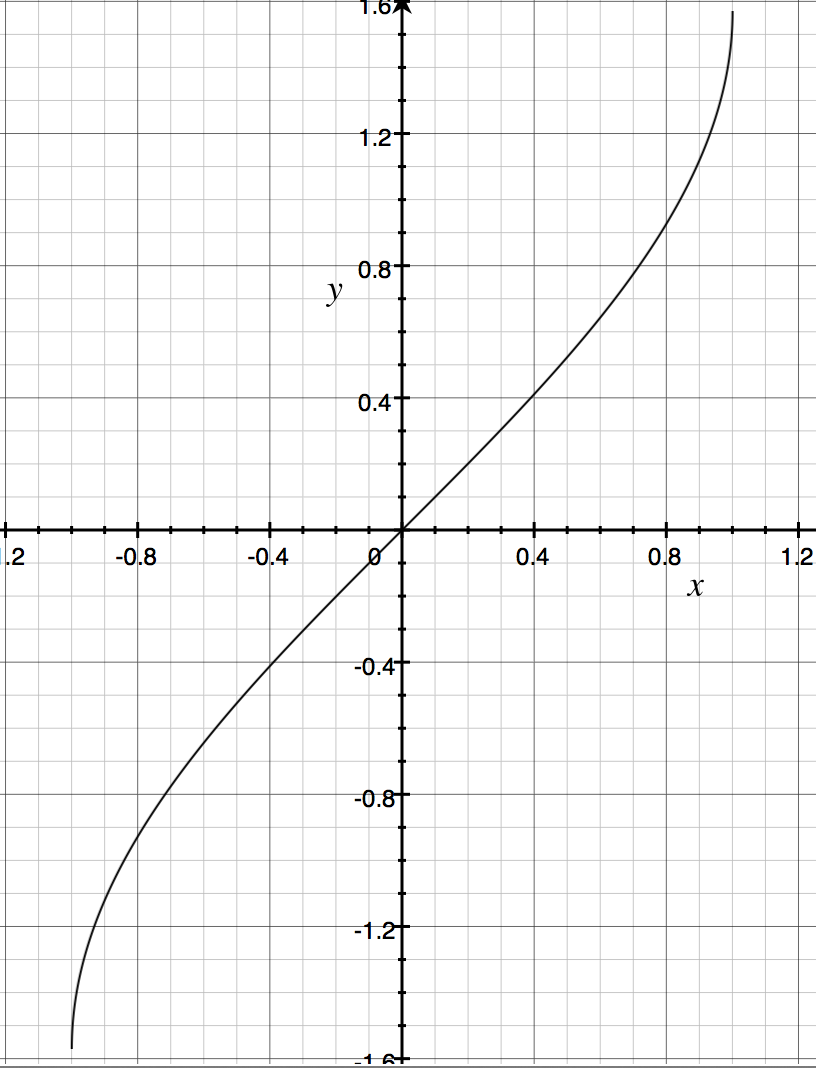
\includegraphics[scale=0.4]{./graphics/arctanx.png}\\
		$\arctan(x)$
	\end{center}
	NOTE: trig functions with caps first letter are informal notation to denote processed sine and cosine functions
	\pagebreak\\
	{\bf Exercises}\\
	Simplify the expression $\cos(\arctan(x))$\\
	\underline{Solution}:
	$$y=\arctan(x)\iff Tan(y)=x \text{ for } y\in~]-\frac{\pi}{2},\frac{\pi}{2}[$$
	On the other hand, we have the trigonometric identity:
	\begin{align*}
		\sec^2(x)&=1+\tan^2(y)\\
		&=1+x^2\text{ why?}
	\end{align*}
	Finally,
	$$
	\cos(\arctan(x))=\cos(y)=\frac{1}{\sec(y)}=\frac{1}{\sqrt{1+x^2}}\text{ ... why?}
	$$
	Compute exactly $\tan(\arcsin(1/3))$\\
	\underline{Solution}\\
	$$
		\theta=\arcsin(1/3)\iff Sin(\theta)=1/3\text{ when }\theta\in~[-\frac{\pi}{2},\frac{\pi}{2}],
	$$
	On the other hand, we  have the trigonometric identity $\cos^2\theta=1-\sin^2\theta$
	\pagebreak\\
	\Large{Limits}\\
	\normalsize
	Let $f:D\rightarrow\mathbb{R}$ be a function, $L\in\mathbb{R}$ and $a\in\mathbb{R}$ a point of either $D$ or a boundary point of $D$.\\
	\underline{Examples of acceptable $a$:}
	\begin{itemize}
		\item If $D=[1,2]$, then $a$ could be 1.5
		\item If $D=]1,3[$ then $a$ could also be 3 or -1, even though they are not in the domain of $f$.
	\end{itemize}
	{\bf Definition:}\\
	We will write:
	$$
		\lim_{x\to a}f:D
	$$
	\underline{Remark:} That value $L$ must be independent of the way we approach $a$.\\\\
	We can expand the definition of limits and ask, "is $f(x)$ approaching a definite value as $|x|$ grows arbitrarily?" We write in this case either:
	$$
		\lim_{x\to \infty}f(x)~~~\text{or}~~~\lim_{x\to-\infty}f(x)
	$$
	In the case of $y=\frac{1}{x}$ we have:
	$$
		\lim_{x\to\infty}f(x)=\lim_{x\to -\infty}f(x)=0
	$$
	{\bf Directional limits}\\
	In some problems, we might be interested in only a certain direction of approach.\\
	If we approach $a$ from the right, we write:
	$$
		\lim_{x\to a^+}f(x)
	$$
	Conversely, if we approach $a$ from the left, we write:
	$$
		\lim_{x\to a^-}f(x)
	$$
	{\bf Theorem:}\\
	The limit $\lim\limits_{x\to a}f(x)$ exists iff both the right and left limit exist and are equal.\\
	
	\noindent Suppose both $\lim\limits_{x\to a}f(x)$ and $\lim\limits{x\to a}g(x)$ are numbers and let $c\in\mathbb{R}$.
	\begin{itemize}
		\item $\lim\limits_{x\to a}(f(x)\pm g(x))=\lim\limits_{x\to a}f(x)\pm\lim\limits_{x\to a}g(x)$
		\item $c\lim\limits_{x\to a}f(x)=\lim\limits_{x\to a}c(f(x))$
		\item $\lim\limits_{x\to a}f(x)g(x)=\left( \lim\limits_{x\to a}f(x) \right)\left( \lim\limits_{x\to a}g(x) \right)$
		\item $\lim\limits_{x\to a}\frac{f(x)}{g(x)}=\frac{\lim\limits_{x\to a}f(x)}{\lim\limits_{x\to a}g(x)}\text{ if }\lim\limits_{x\to a}g(x)\ne 0$
	\end{itemize}
	{\bf Definition}
	Let $f:D\rightarrow\mathbb{R}$ be a function and $a\in D$. We say that $f$ is \emph{continuous at} $a$ if:
	$$
		f(a)=\lim_{x\to a}f(x)
	$$
	{\bf Examples of continuous functions}
	\begin{itemize}
		\item All polynomial functions
		\item All trig functions
		\item All exponential and log functions
		\item All rational functions
	\end{itemize}
	\underline{\bf Warning:} One checks continuity only on $x$ belonging to the domain of a function.\\
	\underline{Question:} Is $\frac{1}{x}$ continuous? Yes, since it is not defined on $x=0$\\\\
	Compute:
	$$
		\lim_{x\to 0}\frac{(3+x)^2-9}{x}
	$$
	Solution: First of all we notice that it is a rational function but 0 is not in its domain. Hence we can't simply substitute 0 in the expression. Thus:
	\begin{align*}
		\lim_{x\to 0}\frac{(3+x)^2-9}{x}&=\lim_{x\to 0}\frac{9+6x+x^2-9}{x}\\
		&=\lim_{x\to 0}\frac{x(6+x)}{x}
	\end{align*}
	As we are interested in the limit when approaching 0, we are purposely avoiding $x=0$, hence:
	$$
		\lim_{x\to 0}\frac{(3+x)^2-9}{x}=\lim_{x\to 0}(6+x)
	$$
	And now we notice that the function $6+x$ is a line (hence continuous) and that 0 is in its domain.\\
	\underline{Conclusion}: $\lim\limits_{x\to 0}\frac{(3+x)^2-9}{x}=\lim\limits_{x\to 0}(6+x)=6+0=6$\\
	Let $f,~g:D\rightarrow\mathbb{R}$ be two continuous functions (when we do not specify at a particular point we mean continuous everywhere on their domain).
	\begin{itemize}
		\item $f\pm g$ is continuous;
		\item $f\cdot g$ is continuous, and
		\item $\frac{f}{g}$ is continuous whenever the quotient is defined, i.e. it is continuous on all $x\in D$ such that $g(x)\ne 0$.	
	\end{itemize}
	Let $f:D\rightarrow\mathbb{R}$ be a continuous function and suppose that there is an interval $[a,b]\subseteq D$\\
 	{\bf Theorem}\\
	For each $y$ between $f(a)$ and $f(b)$, there is $x_0\in[a,b]$ such that $y=f(x_0)$\\
	Suppose that we have a continuous function $f:[0,1]\rightarrow[0,1]$\\
	Then one knows that there is $x_0\in[0,1]$ such that $f(x_0)=x_0$, i.e. $f$ admits a fixed point.\\
	Why?\\
	Consider the new function
	\begin{align*}
		g:[0,1]&\longrightarrow\mathbb{R}\\
		x&\mapsto f(x)-x
	\end{align*}
	On one hand, if $f(1)=1$, then we are done as we have found a fixed point. Else by construction
	$$
		g(1)<0\text{ since }f(1)<1
	$$
	On the other hand, if $f(0)=0$ then again we are done. Else by construction
	$$
		g(0)>0\text{ since }f(0)>0
	$$
	\pagebreak\\
	{\bf General culture}\\
	This result is true in higher dimensions!\\
	It is known as the \emph{Brouwer fixed-point theorem}.\\
	{\bf Theorem:}\\
	Let $f:[0,1]^n\rightarrow[0,1]^n$ be a continuous function for $n=1,2,3,...$. There exists $x_0\in[0,1]^n$ such that:
	$$
		f(x_0)=x_0
	$$\\
	{\bf Second hypothesis}\\
	Let $p(x)=x^n+a_{n-1}x^{n-1}+...+a_1x+a_0$ be a polynomial of odd degree grate or equal to 1, i.e. $n$ can only be an odd positive integer greater than or equal to one.\\
	{\bf Theorem}\\
	One automatically knows that there is at least one $x_0\in\mathbb{R}$ such that
	$$
		p(x_0)=0
	$$
	Why?\\
	Intuitively, we know that
	$$
		\lim_{x\to\pm\infty}p(x)=\lim_{x\to\pm\infty}x^n
	$$
	Moreover, on one hand:
	$$
		\lim_{x\to\infty}x^n=\infty
	$$
	i.e. there is a $b\in\mathbb{R}$ such that $p(b)>0$.\\
	On the other hand, we also know that since $n$ is odd,
	$$
		\lim_{x\to-\infty}x^n=-\infty
	$$
	i.e. there is $a\in\mathbb{R}$ such that $p(a)<0$\\
	Conclusion: By the intermediate value theorem there must exist $x_0\in[a,b]$ such that:
	$$
		p(x_0)=0
	$$\\
	\pagebreak\\
	\Large{The derivative}\\
	\normalsize
	{\bf Outline}
	\begin{enumerate}
		\item Geometric interpretation
		\item The derivative as a function
		\item Computation\\
	\end{enumerate}
	{\bf Recall:}\\
	Let $f:D\rightarrow\mathbb{R}$ be a function and $x_0\in D$.\\\\
	{\bf Definition:}\\
	We say that $f$ is differentiable at $x_0\in D$ if the following limit:
	$$
		\lim_{h\to 0}\frac{f(h+x_0)-f(x_0)}{h}
	$$
	is a number, i.e. it exists.\\
	In that case we denote the number $f'(x_0)$.\\
	The question is, what does it mean to differentiate a function at $x_0$?\\
	Recall how one computes the slope of a line:
	$$
		m=\frac{\Delta y}{\Delta x}
	$$
	Hence in the case of the line $\mathbb{D}$, we have
	$$
		m_{\mathbb{D}}=\frac{f(x_0+\Delta x)-f(x_0)}{\Delta x}
	$$
	Now as $\Delta x$ goes towards 0, the slope $m_D$ goes towards the slope of the red line.\\\\
	{\bf Continuity?}\\
	Suppose $f:D\rightarrow\mathbb{R}$ is differentiable at $x_0\in\mathbb{R}$.\\
	Pick and $x\in D$ but such that $x\ne x_0$. Then
	\begin{align*}
		f(x)&=f(x)+0\\
		&=f(x)-f(x_0)+f(x_0)\\
		&=(f(x)-f(x_0))\cdot 1+f(x_0)\\
		&=(f(x)-f(x_0))\frac{x-x_0}{x-x_0}+f(x_0)\\
		&=\frac{f(x)-f(x_0)}{x-x_0}(x-x_0)+f(x_0)
	\end{align*}
	And now we can take the limit on each side, i.e.
	\begin{align*}
		\lim_{x\to x_0}&=\lim_{x\to x_0}\left(\frac{f(x)-f(x_0)}{x-x_0}(x-x_0)+f(x_0)\right)\\
		&=\left(\lim_{x\to x_0}\frac{f(x)-f(x_0)}{x-x_0}\lim_{x\to x_0}(x_{x_0})+\lim_{x\to x_0}f(x_0)\right)\\
		&=f'(x_0)\cdot 0+f(x_0)\\
		&=f(x_0)
	\end{align*}
	{\bf Conclusion:} $f$ is continuous at $x_0$.\\
	\underline{Warning:} The converse is false, i.e. a continuous function is not necessarily differentiable.\\
	\begin{center}	
		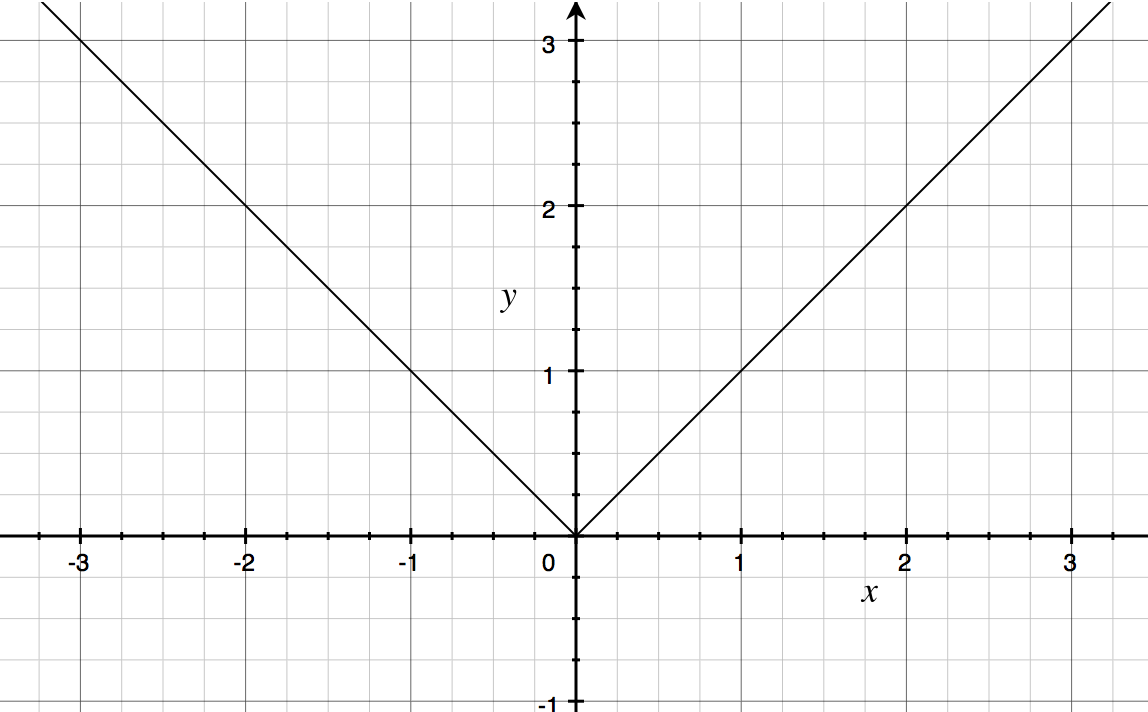
\includegraphics[scale=0.5]{./graphics/absx.png}\\
		$y=|x|$ \emph{is continuous, but not differentiable.}
	\end{center}
	Let $f:D\rightarrow\mathbb{R}$ be a function. Consider the subset
	$$
		C=\{a\in D~|~f'(a)\text{ exists}\}
	$$
	Then one can construct a new function:
	\begin{align*}
		f':C&\rightarrow\mathbb{R}\\
		x&\mapsto f'(x)
	\end{align*}
	If $f(x)=c$, i.e., $f$ is a constant, then
	\begin{align*}
		f'(x)&=\lim_{h\to 0}\frac{f(x+h)-f(x)}{h}\\
		&=\lim_{h\to 0}\frac{c-c}{h}\\
		&=\lim_{h\to 0}\frac{0}{h}=0
	\end{align*}
	Let $n=1,~2,~3,~...$ and consider the function $f(x)=x^n$\\
	Recall the binomial formula:\\
	$$
		(a+b)^n=\left(\begin{array}{c}{n}\\{0}\end{array}\right)a^n+\left(\begin{array}{c}{n}\\{1}\end{array}\right)a^{n-1}b+\left(\begin{array}{c}{n}\\{2}\end{array}\right)a^{n-2}b^2+...+\left(\begin{array}{c}{n}\\{n-1}\end{array}\right)ab^{n-1}+\left(\begin{array}{c}{n}\\{n}\end{array}\right)b^n
	$$
	$$
		=\sum^{n}_{k=0}\left(\begin{array}{c}{n}\\{k}\end{array}\right)a^{n-k}b^k
	$$
	Where $\left(\begin{array}{c}{n}\\{k}\end{array}\right)=\frac{n!}{(n-k)!k!}$
	Then
	\begin{align*}
		f'(x)&=\lim_{h\to 0}\frac{f(x+h)-f(x)}{h}\\
		&=\lim_{h\to 0}\frac{x+h)^n-x^n}{h}\\
		&=\lim_{h\to 0}\frac{ \left[ \sum\limits^n_{k=0}\left(\begin{array}{c}{n}\\{k}\end{array}\right) x^{n-k}h^k \right] -x^n}{h}\\
		&=\lim_{h\to 0}\frac{ \left[ \sum\limits^n_{k=1}\left(\begin{array}{c}{n}\\{k}\end{array}\right) x^{n-k}h^k \right]}{h}\\
		&=\lim_{h\to 0}\left[ \sum\limits^n_{k=1}\left(\begin{array}{c}{n}\\{k}\end{array}\right) x^{n-k}h^{k-1} \right]\\
		&=\left(\begin{array}{c}{n}\\{1}\end{array}\right)x^{n-1}=nx^{n-1}
	\end{align*}
	\pagebreak\\
	\Large{Trigonometry}\\
	\normalsize
	How do your compute the derivative of $y=\sin(x)$?
	\begin{align*}
		\frac{d\sin}{dx}(x)&=\lim_{h\to 0}\frac{\sin(x+h)-\sin(x)}{h}\\
		&=\lim_{h\to 0}\frac{\sin(x)\cos(h)+\sin(h)\cos(x)-\sin(x)}{h}\\
		&=\lim_{h\to 0}\frac{\sin(x)(\cos(h)-1)}{h}+\lim_{h\to 0}\frac{\sin(h)\cos(x)}{h}\\
	\end{align*}
	To help us go beyond those examples, we need "recipes:"\\
	Let $f$ and $g$ two differentiable functions $c\in\mathbb{R}$.
	\begin{itemize}
		\item $(cf)'(x)=cf'(x)$
		\item $(f\pm g)'(x)=f'(x)\pm g'(x)$
		\item $(f\cdot g)'(x)=f'(x)\cdot g(x)+f(x)\cdot g'(x)$
		\item $\left(\frac{f}{g}\right)'(x)=\frac{f'(x)g(x)-f(x)g'(x)}{g(x)^2}$
	\end{itemize}
	Let $f(x)=a^x$ for some $a\in~]0,1[~\cup~]1,+\infty[$
	\begin{align*}
		f'(x)&=\lim_{h\to 0}\frac{a^{x+h}-a^x}{h}\\
		&=\lim_{h\to 0}\frac{a^x(a^h-1)}{h}\\
		&=a^x\left(\lim_{h\to 0}\frac{a^h-1}{h}\right)
	\end{align*}
	\large{\bf The number $e$}\\
	\normalsize
	Let's consider two possible $a$, i.e. $a=2$ and $a=3$, and let's approximate in those two cases the limit
	$$
		\lim_{h\to 0}\frac{a^{h}-1}{h}
	$$
	\begin{center}
		\begin{tabular}{r | c | l}
			{$h$}&{$\frac{2^h-1}{h}$}&{$\frac{3^h-1}{h}$}\\
			{0.1}&{0.7177}&{1.1612}\\
			{0.01}&{0.6956}&{1.1047}\\
			{0.001}&{0.6934}&{1.0992}\\
			{$\vdots$}&{$\vdots$}&{$\vdots$}
		\end{tabular}
	\end{center}
	\underline{Definition:}\\
	The number $e$ is a number between 2 and 3 such that
	$$
		\lim_{h\to 0}=\frac{e^h-1}{h}=1
	$$
	If $f(x)=e^x$, then $f'(x)=e^x$.
	\begin{enumerate}
		\item Tangent line
		\item Velocity
		\item Higher derivatives
	\end{enumerate}
	\large{Equation of a line}\\
	\normalsize
	Recall that the equation of a line in the plane is $y=mx+b$, where $m$ is the slope and $b$ is the height on the y-axis at which the line crosses.\\
	To find the equation of a line one needs the coordinates of two distinct points on that line or a point on the line and its slope. Now if one is given $f'(x_0)$ and the point $(x_0,f(x_0))$, the the equation of the tangent line to the graph of $f$ at the point $x_0$ is given by
	$$
		y=f'(x_0)x+f(x_0)-x_0f'(x_0)
	$$%
	Consider $f(x)=x^2-\sin x$ and give the equation of the tangent line of $f$ at the point $x_0=0$.\\
	We need to compute:
	\begin{itemize}
		\item $f(0)=0$
		\item $f'(0)$. In general, $f'(x^2)=2x$
	\end{itemize}
	\large{velocity}
	Suppose a particle is moving along a straight line. Hence we have a function:
	\begin{align*}
		s:[a,b]&\rightarrow\mathbb{R}\\
		t&\mapsto s(t)
	\end{align*}
	that tracks its position along that line. Its position with respect to the origin at some time $t_0\in[a,b]$ is
	$$
		s(t_0)
	$$
	{\bf Definition}\\
	The \emph{average speed} at which it travelled during the interval of time $[a,b]$ is the ratio of the total displacement $\Delta s=s(b)-s(a)$ by the total time of travel, i.e.
	$$
		\overline{v}=\frac{\Delta s}{\Delta t}=\frac{s(b)-s(a)}{b-a}
	$$
	{\bf Definition}\\
	If the position of a particle is modelled along a differentiable function $s$, then the instantaneous velocity at time $t_0$ is
	$$
		s'(t_0)
	$$
	{\bf Example}\\
	Suppose a man throws a stone upward and that the position once it leaves the hand of the stone with respect to the ground is given by $s(t)=-5t^2+10t+1$
	\begin{itemize}
		\item At what height does the stone leave the hand?
		\item What is the initial velocity of the stone?
		\item What is the maximum height that the stone reaches?
		\item At what velocity does the stone hit the ground?
		\item What is the average velocity of the stone from the time it leaves the hand to when it hits the ground?
	\end{itemize}
	Solutions:
	\begin{itemize}
		\item Set $t=0$ and compute.
		\item $v(t)=s'(t)=-10t+10$, hence $v(0)$=10
		\item Find x-intercept of $v(t)$ and plug x-value into $s(t)$.
		\item Find the root $x_2$ of $s(t)$ and the slope of the tangent at that point.
		\item Find $s(t)$ at $t=0$, and at $t=x_2$, and average.
	\end{itemize}
	{\bf Higher derivatives}\\
	We have seen that from a differentiable function $f$ one can compute its derivative $f'$ which is yet another function. It is then reasonable to ask, "is that new function differentiable?"\\
	Let $y=\sin(x)$, then $y=\cos(x)$. Then, $y''=-\sin(x)$.
	Recall that the derivative at a point measures the instantaneous variation at that point of the original function. That can now be applied to the derivative,i.e. the second derivative at a point measures the instantaneous variation at that point of the derivative.\\
	\begin{enumerate}
		\item Compute the derivative of $f(x)=\frac{1}{x^n}$ for $n=1,2,3$\\
		\begin{align*}
			f'(x)&=\frac{0\cdot x^n-1\cdot nx^{n-1}}{(x^n)^2}\\
			&=-\frac{nx^{n-1}}{x^{2n}}\\
			&=-\frac{n}{x^{2n-n+1}}\\
			&=-\frac{n}{x^{n+1}}
		\end{align*}
		Consider $y=x^a$.\\
		In the case, $a\in\mathbb{Z}$ we have $y'=ax^{a-1}$. This is true, in general.\\
		{\bf Theorem}\\
		For any $a\in\mathbb{R}$, we have
		$$
			y'=ax^{x-1}
		$$
		{\bf Warning}\\
		Even through $\sqrt{x}$ is continuous on its domain, i.e. on $[0,+\infty]$, it is \emph{not} differentiable at 0.\\
		\item Compute the derivative of $y'$ when $y=x^2\cos(x)$
		{\bf Definition:}\\
		We say that a value $M\in\mathbb{R}$ is the maximum of $f$ if there is an $x_0\in D$ such that 
		$$
			M=f(x_0)\ge f(x)~\forall~x\in D
		$$
		Clearly we have its counterpart, i.e., $m\in\mathbb{R}$ is the minimum of $f$ if there is $x_1\in D$ such that
		$$
			m=f(x_1)\le f(x)~\forall~x\in D
		$$
	\end{enumerate}
	Let $f:D\rightarrow\mathbb{R}$ be a function. Suppose that $f$ is differentiable on an open interval. Pick a point $a$ on that open interval.\\
	{\bf Theorem}\\
	If $f$ achieves either a local maximum or a local minimum at $a$, then $f'(a)=0$.\\
	{\bf Warnings}
	\begin{itemize}
		\item The converse is false!
		\item We need $f$ to be differentiable on an open interval $a$.
	\end{itemize}
	{\bf Critical point}\\
	Let $f:D\rightarrow\mathbb{R}$ be a function.\\
	{\bf Definition}\\
	A point $x_0\in D$ is a critical point of $f$ if either
	$$
		f'(x_0)=0\text{ or }f'(x_0)\text{ does not exist}.
	$$
	Example: In the following example, $y=(1-x)x^{1/3}+1$
	$$
		y'=-x^{1/3}+(1-x)\frac{1}{3x^{2/3}}=\frac{1-4x}{3x^{2/3}}
	$$
	\large{Outline}
	\normalsize
	\begin{enumerate}
		\item The chain rule
		\item Implicit differentiation
		\item Differentiating inverse functions
	\end{enumerate}
	\large{\bf The chain rule}\\
	\normalsize
	We need to find a convenient way to differentiate functions of the form
	$$
		\sqrt{x^2+1}\text{ and }e^{-x^2}.
	$$
	Let $f:D\rightarrow\mathbb{R}$ and $g:E\rightarrow\mathbb{R}$ be two functions such that
	$$
		g(E)\subset D.
	$$
	Moreover, suppose that $g$ is differentiable at $x_0\in E$ and that $f$ is differentiable at $g(x_0)$.\\
	{\bf Theorem}
	$$
		(f\circ g)'(x_0)=f'(g(x_0))\cdot g'(x_0)
	$$
	{\bf Examples}
	\begin{itemize}
		\item We can finally compute the derivative of $y=a^x$ for $0<a<1$ or $a>1$.\\
		Recall that $x=e^{\ln x}$.\\
		So, by the rule of exponents we have $y=e^{x\ln a}$.\\
		Consider $g(x)=x\ln a$. Then $y=e^{g(x)}$, hence
		\begin{align*}
			g'&=e^{g(x)}\cdot g'(x)\\
			&=y\cdot\ln a\\
			&=a^x\cdot\ln a
		\end{align*}
		\item Compute the derivative of $y=(x^3-1)^{100}$.\\
		$f(x)=x^3-1$, $g(x)=f(x)^{100}$\\
		$y'=100(x^3-1)^{99}\cdot 3x^2$
		\item Compute the derivative of $y=\left(\frac{t-2}{2t+1}\right)^9$\\
		$f(x)=\frac{t-2}{2t+1}$, $g(x)=f(x)^9$
		\begin{align*}
			y'&=9\left(\frac{t-2}{2t+1}\right)^8\cdot \frac{5}{(2t+1)^2}\\
		\end{align*}
		\item Compute the derivative of $y=\sin(\cos(\tan(x)))$
		\begin{align*}
			y'&=-\cos(\cos(\tan(x)))\cdot\sin(\tan(x))\cdot\sec^2(x)
		\end{align*}
	\end{itemize}
	\large{\bf Implicit differentiation}\\
	If a function $y=f(x)$ verifies a certain relation, then its derivative $y'$ should verify the derivative of the relation.\\
	\underline{Remarks:}
	\begin{itemize}
		\item In such a case it is not uncommon that the actual function is unknown
		\item The existence problem of such a function is beyond this course, i.e., given a relation, is there a function that verifies it? This course assumes that this is the case.
	\end{itemize}
	\large{\bf Examples}
	\normalsize
	\begin{itemize}
		\item Suppose we know that a certain function $y=f(x)$ satisfies the relation $x^3+y^3=6xy$, i.e.
		$$
			x^3+(f(x))^3=6xf(x)
		$$
		{\bf Question:} What is the slope of the tangent line at the point, $(x,y)=(3,3)$?\\
		We first differentiate the relation (1), i.e
		$$
			3x^3+3(f(x))^2\cdot f'(x)=6f(x)+6xf'(x)
		$$
		Using chain rule on the left-hand side and product rule on the right-hand side.
		$$
			f'(x)=\frac{6f(x)-3x^3}{3(f(x))^2-6x}=\frac{2f(x)-x^2}{(f(x))^2-2x}
		$$
	\end{itemize}
	\large{\bf Inverse trig functions}\\
	\normalsize
	What is the derivative of $\arcsin(x)$?\\
	\underline{Solution:} Recall that
	$$
		y=\arcsin(x)\iff\sin(y)=x\text{ AND }-\frac{\pi}{2}\le y\le\frac{\pi}{2}
	$$
	\begin{itemize}
		\item Since $-\frac{\pi}{2}\le y\le\frac{\pi}{2}$, we have $\cos(y)\ge 0$. Moreover,
		$$
			\cos(y)=+\sqrt{1-\sin^2(y)}=\sqrt{1-x^2}
		$$
		\item We now differentiate implicitly the relation $\sin(y)=x$ with respect to  $x$, i.e.
		$$
			\cos(y)\cdot y'=1
		$$
		\underline{Conclusion:}
		$$
			\arcsin'(x)=\frac{1}{\sqrt{1-x^2}}
		$$
		\item Homework: prove that the derivative of $y=\arccos(x)$ is
		$$
			\frac{-1}{\sqrt{1-x^2}}
		$$
		\item What about the derivative of $y=\arctan(x)$?\\
		Solution: Recall that
		$$
			y=\arctan(x)\iff\tan(y)=x\text{ AND }-\frac{\pi}{2}<y<\frac{\pi}{2}
		$$
		\begin{itemize}
			\item Recall that $\tan^2(y)+1=\sec^2(y)$. Hence
			$$
				\sec^2(y)=x^2+1
			$$
		\end{itemize}
		\item We now know how  to differentiate implicitly the relation $\tan(y)=x$ with respect to $x$, i.e.
		$$
			\sec^2(y)\cdot y'=1\text{ (using chain rule)}
		$$
	\end{itemize}
	Suppose the $f:A\rightarrow B$ and $f^{-1}:B\rightarrow A$ are differentiable functions and inverse to each other, i.e.
	$$
		f^{-1}(f(x))=x\text{ and }f(f^{-1}(y))=y
	$$
	for all $x\in A$ and $y\in B$.\\
	If one differentiates the first of these two identities, one gets
	$$
		(f^{-1}\prime(f(x))\cdot f'(x))=1
	$$
	{\bf Example: $\ln(y)$}\\
	We know that $\ln(e^x)=x$ and that the derivative of $y=e^x$ is itself.\\
	Compute the derivative of $y=\ln(\cos(x))$\\
	Solution: It is a composition of functions. Hence we apply the chain rule:
	\begin{align*}
		y'&=\frac{1}{\cos(x)}(-\sin(x))\\
		&=-\tan(x)
	\end{align*}
	\pagebreak
	\large{\bf Logarithmic differentiation}\\
	\normalsize
	Compute the derivative of 
	$$
		y=\frac{x^{3/4}\sqrt{x^2+1}}{(3x+2)^5}
	$$
	Solution: We will combine logarithmic laws and implicit differentiation to compute this.\\
	Start by taking $\ln$ on both sides, i.e.
	\begin{align*}
		\ln y&=\ln\left(\frac{x^{3/4}\sqrt{x^2+1}}{(3x+2)^5}\right)\\
		&=\frac{3}{4}\ln x+\frac{1}{2}\ln(x^2+1)-5\ln(3x+2)\\
		\frac{1}{y}\frac{dy}{dx}&=\frac{3}{4}\cdot\frac{1}{x}+\frac{1}{2}\cdot\frac{2x}{x^2+1}-5\cdot\frac{3}{3x+2}
	\end{align*}
	Now solve for $\frac{dy}{dx}$:
	\begin{align*}
		\frac{dy}{dx}&=y\left(\frac{3}{4x}+\frac{x}{x^2+1}-\frac{15}{3x+2}\right)\\
		&=\frac{x^{3/4}\sqrt{x^2+1}}{(3x+2)^5}\left(\frac{3}{4x} INCOMPLETE \right)
	\end{align*}
	Compute the derivative of $y=x^{\sqrt{x}}$\\
	$$
		\ln y=\ln x^{\sqrt{x}}=\sqrt{x}\ln x
	$$
	We now differentiate implicitly and use the product rule, namely:
	$$
		\frac{y'}{y}=\frac{1}{2\sqrt{x}}\ln x+\sqrt{x}\frac{1}{x}
	$$
	And solve for $y'$:
	$$
		y'=y\left(\frac{\ln x}{2\sqrt{x}}+\frac{1}{\sqrt{x}}\right)
	$$
	\large{Linear approximation}\\
	Suppose there is an engineer at the train station on the departing deck who wants ot measure the length of the train as it is leaving the station. Of course, this engineer is equipped with a state of the art laser measuring tool. Einstein tells us that the length $\tilde{\mathcal{L}}$ is scaled by a factor of
	$$
		\sqrt{1-\frac{v^2}{c^2}}
	$$
	We can, with a high degree of confidence use linear approximation.
	\begin{align*}
		\tilde{\mathcal{L}}=\mathcal{L}\sqrt{1-\frac{v^2}{c^2}}&\approx L\left(1-\frac{1}{2}\frac{v^2}{c^2}\right)\\
		INCOMPLETE
	\end{align*}
	Suppose that the speed of the train is $v=0.95c$, i.e. 95\% of the speed of light. Then the ratio
	$$
		\frac{v^2}{c^2}=(0.95)^2=0.9025
	$$
	can no longer be considered close to 0.\\
	If you insist on using the linear approximation you would predict a contraction of
	\begin{align*}
		\tilde{\mathcal{L}}&\approx \mathcal{L}\left(1-\frac{1}2\frac{v^2}{c^2}\right)
	\end{align*}
	Physics engineers when fine-tuning cyclotrons are faced with "heavy" electrons. These are electrons accelerated to near the speed of light. Their masses are given by
	$$
		\tilde{m}=\frac{m}{\sqrt{1-\frac{v^2}{c^2}}}
	$$
	\large{Linear approximation (cont'd)}\\
	\normalsize
	Suppose we have a differentiable function $f:D\rightarrow\mathbb{R}$ such that both $f(a)$ and $f'(a)$ are known.\\
	Then, the linear approximation of $f$ at $a$ is
	$$
		L_a(x)=f'(a)(x-a)+f(a)
	$$
	We often write
	$$
		f(a+\Delta x)\approx L_a(a+\Delta x)
	$$
	{\bf Example:}\\
	Find the linear approximation to $f(x)=\sqrt{x+3}$ in the neighbourhood of $a=1$. Then use that approximation to estimate $\sqrt{3.98}$ and $\sqrt{4.02}$.\\
	Solution: We need to compute both $f(1)$ and $f'(1)$, i.e.
	\begin{itemize}
		\item $f(1)=\sqrt{1+3}=2$
		\item $f'(x)=\frac{1}{2\sqrt{x+3}}$. Hence, $f'(1)=\frac{1}{4}$.
	\end{itemize}
	Conclusion: The linear approximation is
	$$
		L_1(x)=\frac{x-1}{4}+2
	$$
	Let's first compute an estimate of $\sqrt{3.98}$.
	\begin{align*}
		\sqrt{3.98}=\sqrt{0.98+3}&=f(0.98)\\
		&\approx L_1(0.98)=\frac{0.98-1}{4}+2=1.995
	\end{align*}
	The real value is $\sqrt{3.98}\approx 1.99499371$\\
	Finally we proceed along the same line of thought to estimate $4.02$.
	\begin{align*}
		\sqrt{4.02}=\sqrt{1.02+3}&=f(1.02)
		&\approx L_1(1.02)=\frac{1.02-1}{4}+2=2.005
	\end{align*}
	The actual value is $\sqrt{4.02}\approx 2.00499376$\\
	\large{Errors under control}\\
	Idea: Suppose you make a measurement $a$ (e.g. length, mass, ...). Clearly there is an associated error $\Delta x$ coming from you, the human, and/or coming from the actual instrument. With this measurement you want to compute a value $f(1)$ (e.g. area, volume, ...).\\
	Question: given that error $\Delta x$ on your measurement, what is the error on the computed value $f(a)$?\\
	One hopes that you are a competent technician and that your company is providing good quality instruments, i.e. $\Delta x$ is small!\\
	Under that hypothesis, one can estimate the error as being INCOMPLETE\\
	Suppose you measure the radius of a sphere and you obtain $r=(21\pm 0.05)cm$. If you use that measurement to compute the volume of the sphere, estimate the error on the computed volume.\\
	Solution: Here, $\Delta r=0.05$. Now recall that the volume of a sphere is $V=\frac{4}{3}\pi r^3$.\\
	The derivative is $4\pi r^2$. Hence the first error to first order is
	$$
		\Delta V\approx|V'(21)|\cdot 0.05=277.1cm^3
	$$
	Have we lost control over that error?\\
	{\bf Definition}\\
	The relative error on a measured or computed value $y$ is
	$$
		\frac{\Delta y}{y}
	$$
	In our example, the relative error on the volume is
	$$
		\frac{|V'(21)|\Delta r}{V(21)}=\frac{4\pi(21)^2 INCOMPLETE}{}
	$$
	While the relative error on the measurement of the radius is $\frac{\Delta r}{r}=\frac{0.05}{21}=0.0024$, or a 0.24\% error.\\
	WARNING: In general, the more computations you do with a single measurement, the more the error will increase.\\
	\large{Related Rates}\\
	\begin{enumerate}
		\item One is inflating a spherical balloon at a rate of $100cm^3/s$. At what speed is the radius increasing when the diameter hits $50cm$?\\
		Solution: Both the volume, $V(t)$, and the radius $r(t)$, of the balloon are functions of time.
		\begin{itemize}
			\item What we know is that $\frac{dV}{dt}=100cm^3/s$
			\item What we are looking for is INCOMPLETE
		\end{itemize}
		The volume and radius are related obviously by
		$$
			V=\frac{4}{3}\pi r^3
		$$
		Hence,
		$$
			\frac{dV}{dt}=4\pi r^2\cdot\frac{dr}{dt}\text{ by the chain rule.}
		$$
		Conclusion:
		\begin{align*}
			\left.\frac{dr}{dt}\right|_{r=25cm}=\frac{1}{4\pi(25)^2}\frac{dV}{dt}\\
		\end{align*}
	\end{enumerate}
		\pagebreak
	\begin{enumerate}
		\item Optimization
		\item Second derivative tests
		\item Optimization problems
	\end{enumerate}
	\normalsize
	This lecture follows closely the one given on September $25^{\text{th}}$ about "What is $f'$ saying?" (absolute min/max vs local min/max).\\
	The idea here is, given a function $f:D\rightarrow\mathbb{R}$, how do we find its maximum or minimum value?\\
	Bur before jumping head on into computations, one needs to check if such computations have any chance to end up with a reasonable answer.\\\\
	\large{\bf Extreme value theorem}\\
	\normalsize
	Suppose the function $f:[a,b]\rightarrow\mathbb{R}$ is continuous and defined on a \underline{closed} interval. Then there exist $c,d\in[a,b]$ such that
	$$
		f(x)\le f(x)\le f(d)~\forall x\in[a,b]
	$$
	{\bf Recall Fermat's Theorem:}\\
	Let $f:D\rightarrow\mathbb{R}$ be a function and a point $c\in~]a,b[~\subset D$.\\
	If $f$ has a local maximum or minimum at $c$, then $c$ is a critical point of $f$, i.e. either $f'(x)=0$ or $f'(c)$ does not exist. A turning point may also be a critical point.\\
	Given a continuous function $f:[a,b]\rightarrow\mathbb{R}$ follow the following steps to find its maximum/minimum value:
	\begin{enumerate}
		\item Find the values of $f$ at all its critical points within $]a,b[$
		\item Compute $f(a)$ and $f(b)$
		\item The largest/smallest values from (1) and (2) will be the maxima/minima of $f$
	\end{enumerate}
	{\bf Example}\\
	Find the maximum and minimum values of the function $f(x)=\frac{x}{x+1}$ on the interval $[1,2]$.\\
	\underline{Solution:} The function is a rational function well-defined on $[1,2]$ and is thus continuous. Hence we now that it achieves its maximum and minimum values.
	\begin{itemize}
		\item To find its critical points, we need its derivative:
		$$
			f'(x)=\frac{1}{(x+1)^2}
		$$
	\end{itemize}
	From our computation, we see that $f'(x)$ is never zero and is well defined on $[1,2]$. Hence $f$ does not have any critical points.
	\begin{itemize}
		\item f(1)=1/2\text{ and }f(2)=2/3
	\end{itemize}
	\underline{Conclusion:} The maximum is 2/3 and the minimum is 1/2.\\\\
	\large{\bf Second derivative}\\
	\normalsize
	Let $f:D\rightarrow\mathbb{R}$\\
	Recall that
	\begin{itemize}
		\item If $f'>0$ on $I$, then $f$ is increasing on $I$; and
		\item If $f'<0$ on $I$, then $f$ is decreasing on $I$
	\end{itemize}
	That gives us a way to determine the concavity of $f$, namely
	\begin{itemize}
		\item If $f''>0$ on $I$, then $f$ is concave up on $I$; and
		\item If $f''<0$ on $I$, then $f$ is concave down on $I$; and
	\end{itemize}
	Let $f:D\rightarrow\mathbb{R}$ be a function and suppose $f'(c)=0$. Is it a local minimum/maximum?\\
	{\bf Theorem}\\
	Suppose there exists and open interval $]a,b[$ such that $c\in~]a,b[~\subset D$. Then
	\begin{itemize}
		\item If $f''>0$ on $]a,b[$, then $f(c)$ is a local minimum.
		\item If $f''<0$ on $]a,b[$, then $f(c)$ is a local maximum.
	\end{itemize}
	\large{\bf Inflection points}\\
	\normalsize
	Let $f:D\rightarrow\mathbb{R}$ be a function.\\
	{\bf Definition:}\\
	A point $c\in D$ is called an inflection point of $f$ if the concavity of $f$ changes at that point.\\\\
	\Large{Optimisation}
	\normalsize
	\begin{enumerate}
		\item Find the closest point on the parabola $y^2=2x$ to the point (1,4).\\
		\underline{Solution:} Recall that the distance between the point (1,4) and an arbitrary point $(x,y)$ is given by
		$$
			d=\sqrt{(x-1)^2+(y-4)^2}
		$$
		Hence we need to minimize $d$ knowing that the point $(x,y)$ that we are looking for satisfies $y^2=2x$\\
		Let's differentiate both $d$ and $y^2=2x$ implicitly with respect to $x$. Namely
		\begin{align*}
			d'&=\frac{1}{2\sqrt{(x-1)^2+(y-4)^2}}\cdot(2(x-1)+2(y-4)\cdot y')\\
			&=\frac{(x-1)+(y-4)y'}{\sqrt{(x-1)^2+(y-4)^2}}
		\end{align*}
		and
		$$
			2y\cdot y'=2
		$$
		Now substituting $y'=1/y$ into $d'$, we get
		$$
			d'=\frac{(x-1)+(1-4/y)}{\sqrt{(x-1)^2+(y-4)^2}}
		$$
		Hence the critical points are given by
		$$
			0=(x-1)+(1-4/y)\text{ or equivalently }xy=4
		$$
		But we need to remember that $y^2=2x$. Hence $y^3=8$, i.e.
		$$
			y=2\text{ and }x=2
		$$
		Verification:
		\begin{itemize}
			\item $d(2,2)=\sqrt{(2-1)^2+(2-4)^2}=\sqrt{5}$
			\item $d(0,0)=\sqrt{(0-1)^2+(0-4)^2}=\sqrt{17}$
		\end{itemize}
		\item Compute the area of the biggest rectangle inscribed into a semicircle of radius $r$.\\
		We know that
		\begin{itemize}
			\item $x^2+y^2=r^2$
			\item $A_{rec}=2x+y$
			\item $0\le x,y\le r$
		\end{itemize}
		Hence we can write
		$$
			A_{rec}(x)=2x\sqrt{r^2-x^2}
		$$
		and we notice that the domain is $[0,r]$ and that $A_{rec}$ is continuous on it. We can apply the algorithm to determine the biggest area.
		\begin{align*}
			A'_{rec}(x)&=2\sqrt{r^2-x^2}+\frac{2x\cdot(-2x)}{2\sqrt{r^2-x^2}}\\
			&=\frac{2(r^2-2x^2)}{\sqrt{r^2-x^2}}
		\end{align*}
		Hence $A'_{rec}(x)=0\iff x=\frac{r}{\sqrt{2}}$.\\
		In that case, $A_{rec}(\frac{r}{\sqrt{2}}=r^2$\\
		$A_{rec}(0)=A_{rec}(r)=0$\\
		{\bf Conclusion:} The biggest inscribed rectangle has an area of $r^2$
	\end{enumerate}
	\Large{l'Hospital's Rule}\\
	\normalsize
	The idea is to find a way to determine certain limits, e.g.
	$$
		\lim_{x\to 1}\frac{\ln x}{x-1},~~~\lim_{x\to\infty}\frac{e^x}{x^2}~~~\text{or}~~~\lim_{x\to 0^+}x^x
	$$
	These are examples of indeterminate forms of the type
	$$
		\frac{0}0,~~~\frac{\infty}\infty,~~~0^0
	$$
	{\bf The hypothesis}\\
	Let $f,g:D\rightarrow\mathbb{R}$ be two differentiable functions and suppose that $g'(x)\ne 0$ in a neighbourhood of a point $a\in D$ (but it could be zero at $a$). Moreover, suppose that either
	$$
		\lim_{x\to a}f(x)=\lim_{x\to a}g(x)=0
	$$
	or
	$$
		\lim_{x\to a}f(x)=\pm\infty~~~\text{and}~~~\lim_{x\to a}g(x)=\pm\infty
	$$
	{\bf Theorem}
	$$
		\lim_{x}\frac{f(x)}{g(x)}=\lim_{x\to a}\frac{f'(x)}{g'(x)}
	$$
	{\bf Remark:} The notation $x\to a$ can be replaced by $x\to\pm\infty$ or $x\to a^{\pm}$\\
	\begin{enumerate}
		\item Compute $\lim_{x\to 0^+}x^x$\\
		{\bf Solution:} This is an indeterminate form of the type $0^0$. Hence we cannot directly apply the rule. But on one hand,
		$$
			x^x=e^{\ln x^x}=e^{x\cdot\ln x}
		$$
		On the other hand, recall the definition of continuity, i.e.
		$$
			\lim_{x\to a}f(x)=f\left(\lim_{x\to a}x\right)=f(a)
		$$
		Whence
		$$
			\lim_{x\to 0^+}x^x=\lim_{x\to 0^+}e^{x\cdot\ln x}
		$$
		$$
		f(x)=e^{\left(\lim_{x\to 0^+}x\cdot\ln x\right)}
		$$
		$$
			e^0=1
		$$
	\end{enumerate}\pagebreak
	\Large{Newton's method}\\
	\large{The problem}\\
	\normalsize Suppose for a given function $f:D\rightarrow\mathbb{R}~\exists~x_0\in D$ such that
	$$
		f(x_0)=0,
	$$
	i.e. the function admits a root (we may have to deduce this from the intermediate value theorem for example).\\
	{\bf Question:} How can $x_0$ be found?\\
	{\bf Degree 1 case:} Suppose $f(x)=ax+b$ with $a\ne 0$. Then
	$$
		x_0=\frac{-b}{a}
	$$
	{\bf Degree 2 case:} Suppose $f(x)=ax^2+bx+c$ with $a\ne 0$ and $\Delta=b^2-4ac\ge 0$. Then we know that
	$$
		x_0=\frac{-b\pm\sqrt{b^2-4ac}}{2a}
	$$
	{\bf Degree 3 case:} A formula using only $n$th-root functions for solving the cubic was given in the $16^{th}$ century by Cardano. See https://en.wikipedia.org/wiki/Cubic\_function .\\
	{\bf Degree 4 case:} A formula using only $n$th-root function for solving the quartic was given in the $16^{th}$ century by Ferrari. See https://en.wikipedia.org/wiki/Quartic\_function .
	{\bf What about degree 5 and above?}\\
	In the $19^{th}$ century Galois showed that there does not exist such a formula involving only $n$th-root functions to solve in general quintic function.\\
	{\bf The general case}\\
	Let $f:D\rightarrow\mathbb{R}$ be a function and $x_1\in D$ a first "guess", i.e. an initial approximation to the actual root $x_0$ of $f$. We will also make the assumption that $f$ is differentiable. Let's replace $f$ by its linear approximation at $x_1$, i.e.
	$$
		f(x)\approx L_{x_1}(x)=f'(x_1)(x-x_1)+f(x_1)
	$$
	Now, instead of searching for $x_0$ such that $f(x_0)=0$, let's find and $x_2$ INCOMPLETE.\\
	Now the hope is twofold:
	\begin{itemize}
		\item The point $x_2$ is in $D$, and
		\item The point $x_2$ is closer to $x_0$ than $x_1$
	\end{itemize}
	If both turn out to be true, we could then iterate the process, i.e. we could compute an $x_3$ as
	IMCOMPLETE\\
	{\bf Theorem}\\
	If the derivative $f'$ of $f$ is continuous and that $f'(x_0)\ne 0$, then there exists a neighbourhood of INCOMPLETE.
	\pagebreak
	\Large{Integration}\\
	\large{Introduction}\\
	\normalsize
	We are going to take our first step towards understanding one of the most important theorems in mathematics, classical mechanics, and electromagnetism.\\
	The implications of this result are felt throughout science and engineering.\\
	It will occupy the remainder of this course, half of MAT1322, and all of MAT2322.\\
	{\bf Stokes' theorem}\\
	{\bf Theorem}
	\Large$$
		\int_{\partial\mathcal{O}}f=\int_{\mathcal{O}}df
	$$
	\normalsize
	We will restrict ourselves to the following case:
	\begin{itemize}
		\item $f:D\subset\mathbb{R}\rightarrow\mathbb{R}$ differentiable
		\item $df=f'$
		\item $\mathcal{O}=[a,b]\subset D$
		\item $\partial\mathcal{O}=\{a\}\cup\{b\}$
		\item $\int_{\partial\mathcal{O}}=INCOMPLETE$
	\end{itemize}
	{\bf The fundamental theorem}\\
	Hence we will try to understand the following:\\
	{\bf Theorem}
	$$
		f(b)-f(a)=\int_{[a,b]}f'
	$$
	Hence our object of study becomes
	$$
		\int_{[a,b]}f'
	$$
	which is a number!\\
	
\end{document}